\section{Analisi}
\label{sec:analisi}
In questa sezione verrà effettuata un'analisi sui risultati mediati su 30 simulazioni,
comparando il modello base con il modello esteso e infine con un modello allo stato dell'arte.

\subsection{Modello Base}
Nelle figure \ref{fig:analisi-base-evacuated} e \ref{fig:analisi-base-casualties} vengono mostrate le percentuali di evacuati
e di morti nel tempo al variare del numero di auto e pedoni.
%
Come si può notare dalla figura \ref{fig:analisi-base-evacuated}, il numero di pedoni non influenza la percentuale di pedoni evacuati nel tempo.
%
Per quanto riguarda le auto, più è alto il numero di auto più tempo è richiesto per evacuare e inoltre più bassa è la percentuale di auto evacuate alla fine della simulazione.
%
Osservando la percentuale di evacuati totali si può notare che un numero minore di auto permette di evacuare il numero maggiore di agenti.
I casi con probabilità di pedoni del 75\% e 100\% si ottiene la stessa percentuale massima di agenti evacuati,
tuttavia il caso con probabilità 75\% ha un andamento più veloce per la presenza delle auto.

\begin{figure}[ht]
    \centering
    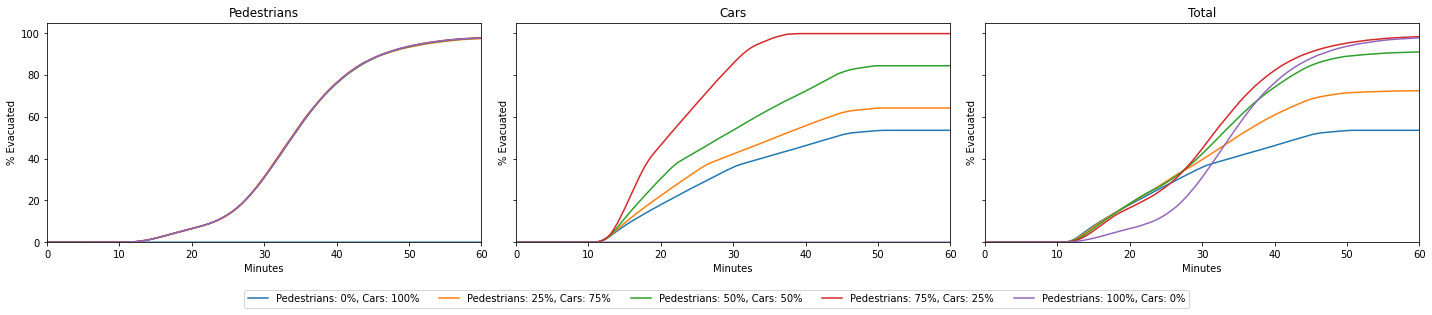
\includegraphics[width=\textwidth]{images/analisi/base-evacuated.png}
    \caption{Percentuale degli evacuati nel tempo al variare del numero di agenti con il modello base.}
    \label{fig:analisi-base-evacuated}
\end{figure}

Per quanto riguarda le percentuali di mortalità (Fig. \ref{fig:analisi-base-casualties}), possono essere fatte analisi simili a quelle in precendenza
per il numero di evacuati.
Per i pedoni in tutti i casi la percentuale di vittime rimane sotto al 1\%, mentre osservando le auto e le vittime totali
risulta una mortalità maggiore all'aumentare del numero di auto fino a un massimo di circa 39\%.
I casi con meno vittime sono quelli con probabilità di auto del 25\% e quello con solo pedoni, che hanno risultati molto simili.

\begin{figure}[ht]
    \centering
    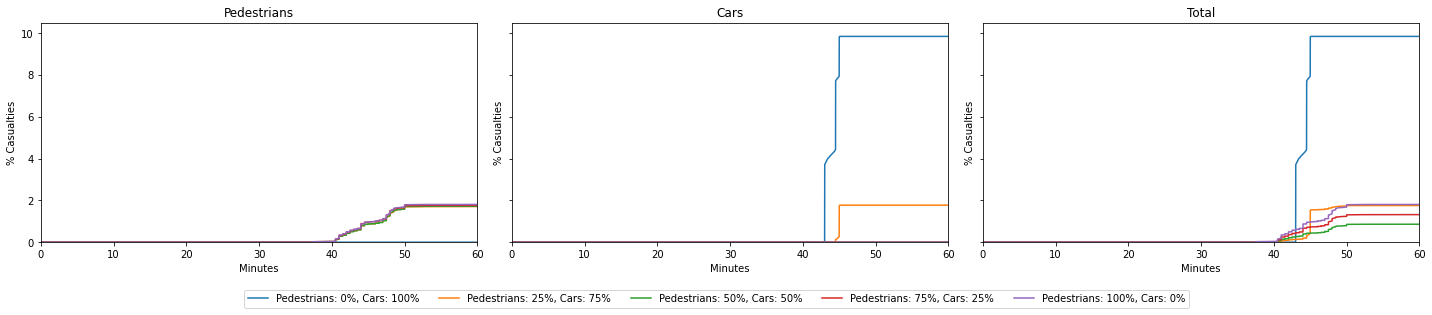
\includegraphics[width=\textwidth]{images/analisi/base-casualties.png}
    \caption{
        Percentuale delle vittime nel tempo al variare del numero di agenti con il modello base.
        %
    }
    \label{fig:analisi-base-casualties}
\end{figure}

Nella figura \ref{fig:analisi-base-evtimes} vengono riportate le percentuali di agenti evacuati nel tempo e il tempo in cui evacuano in media.
%
Nel caso con solo pedoni si ha un picco a 31 minuti che corrisponde al tempo medio di evacuzione.
All'aumentare del numero di auto il tempo medio si abbassa fino a 20 minuti nel caso con solo auto.

Nel caso con probabilità di auto del 25\% sembra formarsi un secondo picco più basso nei primi minuti probabilmente dovuto alle auto, mentre il secondo ai pedoni.
Questi picchi tendono ad appiattirsi con l'aumentare del numero di auto.

Inoltre si può notare come con un numero maggiore di auto considerate la percentuale di agenti che evacuano negli ultimi minuti sia più bassa.
Questo poiché, come già evidenziato nella figura \ref{fig:analisi-base-evacuated}, le auto evacuano più velocemente dei pedoni.

\begin{figure}
    \centering
    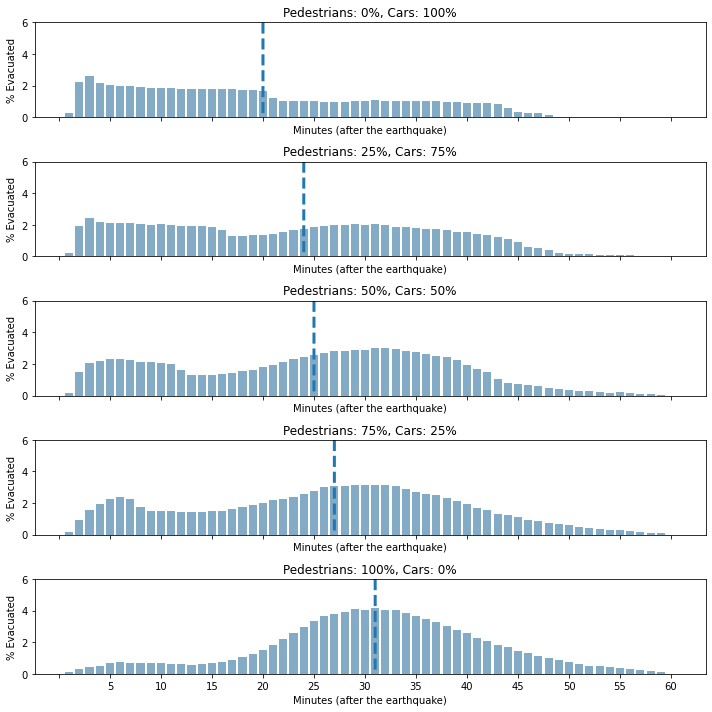
\includegraphics[width=\textwidth]{images/analisi/base-evtimes.png}
    \caption{
        Distribuzione del tempo di evacuzione in percentuale al variare del numero di agenti e tempo medio di evacuazione.
    }
    \label{fig:analisi-base-evtimes}
\end{figure}

\pagebreak

\subsection{Modello Esteso}
Nonostante l'introduzione della variazione della velocità per i pedoni,
la percentuale di pedoni evacuati risulta molto simile al variare del numero di pedoni (Fig. \ref{fig:analisi-new-evacuated}).
Si può notare una piccola differenza tra il minuto 25 e il minuto 35 per il caso con solo pedoni in cui l'andamento è leggermente più basso.

Il caso con solo auto, al contrario di come si possa pensare, non è il caso peggiore e ha un numero di evacuati simile ai casi
con probabilità di auto di 75\% e 50\%, mentre il caso con una percentuale maggiore è quello con una probabilità del 25\%.

In generale il numero di auto evacuate è molto più basso rispetto a quello dei pedoni.

Considerando i contributi di auto e pedoni, al diminuire del numero di auto il numero totale di evacuati alla fine della simulazione cresce,
fino al caso migliore con solo pedoni.

\begin{figure}[ht]
    \centering
    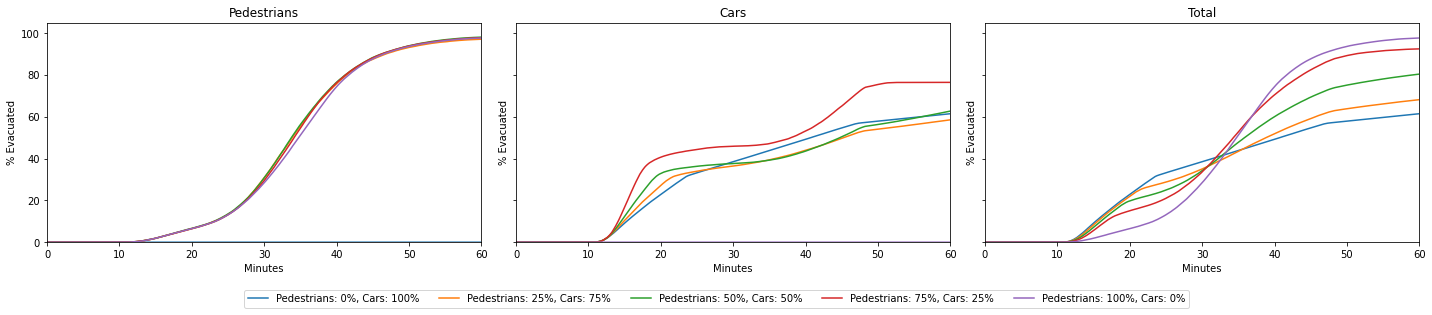
\includegraphics[width=\textwidth]{images/analisi/new-evacuated.png}
    \caption{Percentuale degli evacuati nel tempo al variare del numero di agenti con il modello esteso.}
    \label{fig:analisi-new-evacuated}
\end{figure}

Come si può vedere nella figura \ref{fig:analisi-new-casualties}, al variare del numero di pedoni considerati non ci sono differenze significative,
mentre per le auto la percentuale di vittime sale al crescere del numero di auto considerate.

In generale la percentuale di vittime per le auto è molto più alta rispetto a quella dei pedoni
con un massimo di poco più del 45\% nel caso con una probabilità di auto del 75\% che risulta con una mortalità superiore anche al caso solo auto.
%
Il numero di vittime totali aumenta al crescere del numero di auto e il caso con solo auto è quello con la percentuale di mortalità maggiore.

\begin{figure}[ht]
    \centering
    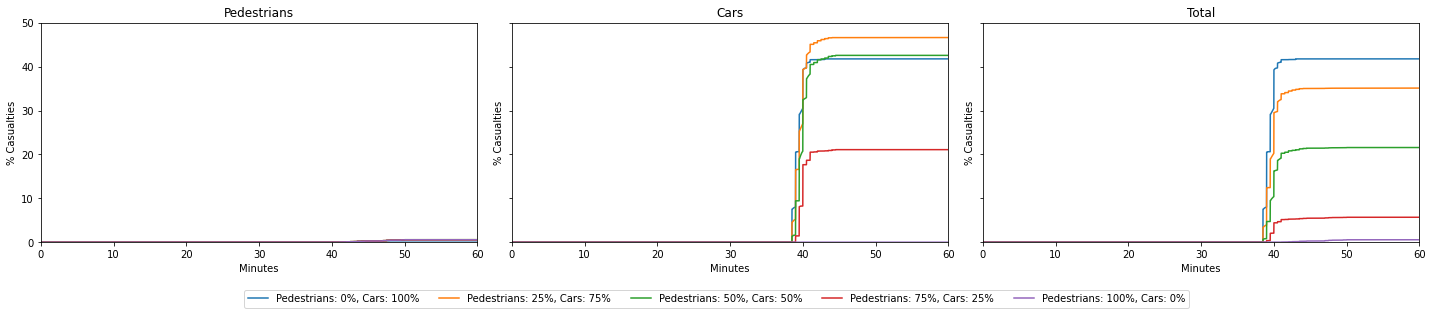
\includegraphics[width=\textwidth]{images/analisi/new-casualties.png}
    \caption{Percentuale delle vittime nel tempo al variare del numero di agenti con il modello esteso.}
    \label{fig:analisi-new-casualties}
\end{figure}

\pagebreak

Nella figura \ref{fig:analisi-new-evtimes} vengono riportate le percentuali di agenti evacuati nel tempo
e il tempo in cui evacuano in media.
%
In modo analogo al modello base il tempo medio di evacuazione si abbassa e sembrano formarsi due picchi nel caso con una probabilità di auto del 25\% per poi appiattirsi
all'aumentare del numero di auto.


\begin{figure}
    \centering
    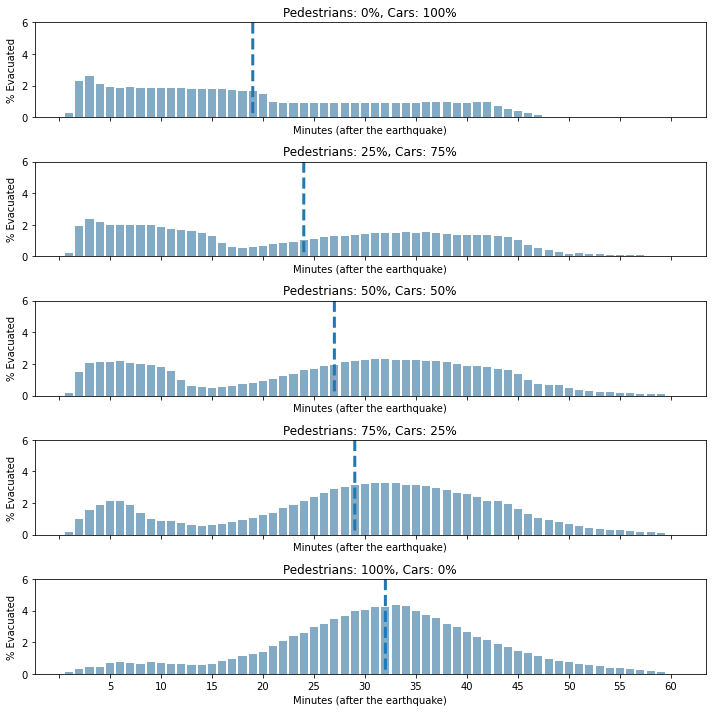
\includegraphics[width=\textwidth]{images/analisi/new-evtimes.png}
    \caption{Distribuzione del tempo di evacuzione in percentuale al variare del numero di agenti e tempo medio di evacuazione.}
    \label{fig:analisi-new-evtimes}
\end{figure}

\pagebreak

\subsection{Comparazione Modello Base e Modello Esteso}
In questa sottosezione verrano comparati il modello base e il modello esteso analizzando
le percentuali di evacuati e di vittime per poi passare a comparazioni spaziali,
in particolare mostrando l'effetto della gestione delle intersezioni durante la simulazione.

\subsubsection*{Percentuale di Evacuati e di Vittime}

\begin{figure}[ht]
    \centering
    \begin{subfigure}{0.45\textwidth}
        \centering
        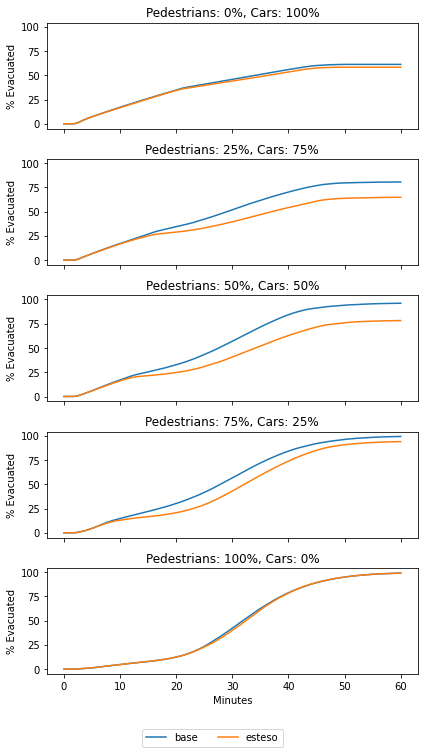
\includegraphics[width=\textwidth]{images/analisi/comparison-total-evacuated.png}
    \end{subfigure}
    \hfill
    \begin{subfigure}{0.45\textwidth}
        \centering
        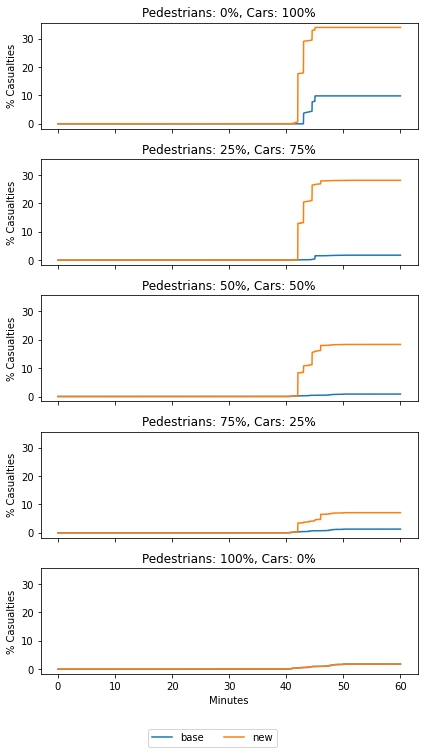
\includegraphics[width=\textwidth]{images/analisi/comparison-total-casualties.png}
    \end{subfigure}
    \caption{Comparazione tra modello base e modello esteso delle percentuali di evacuati (sinistra) e di vittime (destra) al variare del numero di agenti.}
    \label{fig:analisi-comparison-total-ec}
\end{figure}

Osservando la figura \ref{fig:analisi-comparison-total-ec} è possibile comparare le percentuali di evacuati e di vittime nel tempo al variare del numero di agenti tra i due modelli.
In generale il modello esteso presenta un numero minore di evacuati e un numero maggiore di vittime rispetto al modello base.
Questo può essere sintomo dell'effetto delle intersezioni che creando rallentamenti causano una mortalità maggiore,
infatti la percentuale di evacuati del modello esteso presenta un andamento più lento rispetto al modello di partenza.

Per entrambi i modelli all'aumentare del numero di auto considerate, la percentuale di evacuati diminuisce e la percentuale di vittime aumenta.
Inoltre per entrambi i modelli le prime vittime si verificano poco prima di 40 minuti.

Gli unici casi in cui il modello esteso e quello base hanno risultati molto simili sono il caso con solo pedoni e il caso solo auto.
Per quanto riguarda il secondo caso, l'effetto delle intersezioni è minimo rispetto a quanto ci si potrebbe aspettare.


\subsubsection*{Percentuale di Evacuati nel Tempo}

Come già detto in precedenza le distribuzioni della percentuale di evacuati nel tempo del modello base e del modello esteso
presentano un andamento simile, in particolare il caso con solo auto (Fig. \ref{fig:analisi-comparison-evtimes}).

La percentuale di evacuati nei casi con sia auto che pedoni nel modello esteso risulta più bassa nella prima metà
della simulazione e più alta dopo.

Il tempo medio di evacuazione per il modello esteso risulta leggermente più alto soprattutto nei casi con più pedoni.
Questo probabilmente è dovuto al fatto che i pedoni hanno la precedenza negli incroci e hanno velocità velocità variabile, a differenza del modello base.


\begin{figure}[ht]
    \centering
    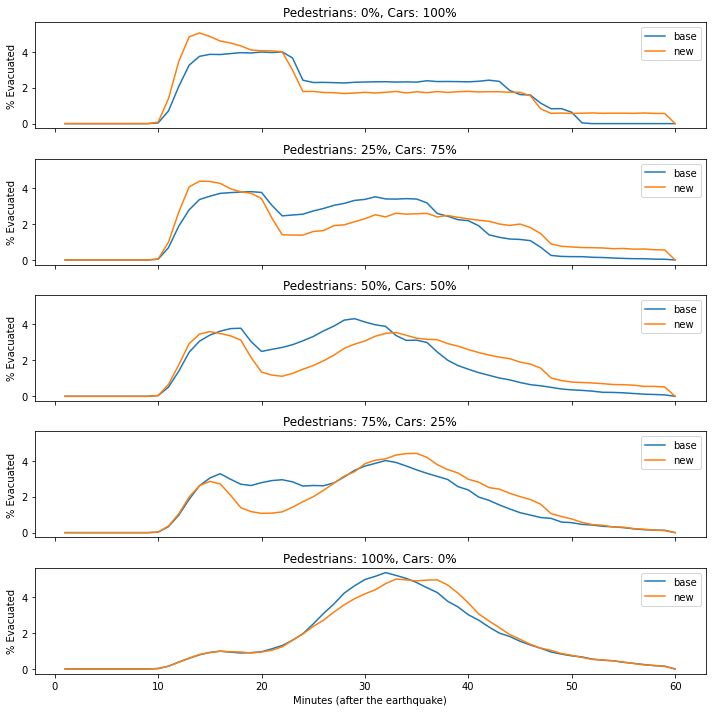
\includegraphics[width=0.9\textwidth]{images/analisi/comparison-evtimes.png}
    \caption{Comparazione delle distribuzioni dei tempi di evacuazione al variare del numero di agenti.}
    \label{fig:analisi-comparison-evtimes}
\end{figure}

\pagebreak

\subsubsection*{Tempo Impiegato per Evacuare}
Un'ulteriore comparazione riguarda il tempo che impiegano auto e pedoni per evacuare.
Come mostrato nella figura \ref{fig:analisi-comparison-evtimes2} per quanto riguarda le auto,
il modello base presenta un andamento decrescente per il tempo medio richiesto per evacuare al diminuire del numero di auto considerate.
Le auto impiegano in media tempi più alti con il modello esteso rispetto a quello base, in particolar modo considerando un numero maggiore di pedoni.
%
I pedoni invece non presentano alcun cambiamento significativo al variare del numero di agenti e del modello considerato.

Per entrambi i modelli un pedone impiega in media un tempo di 25 minuti per evacuare e un massimo di 47 minuti.
Per le auto invece il tempo medio di evacuazione per il modello base è 12 minuti e per il modello esteso 16 minuti,
con tempi massimi rispettivamente di 47 e 48 minuti.

\begin{figure}[ht]
    \centering
    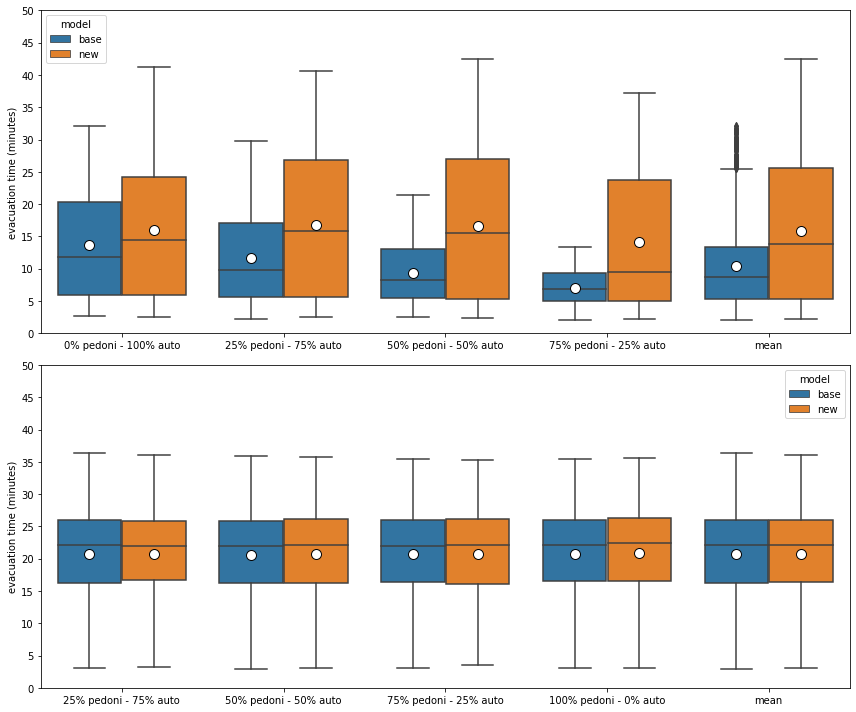
\includegraphics[width=\textwidth]{images/analisi/comparison-evtimes2.png}
    \caption{
        Comparazione dei tempi di evacuazione al variare del numero di agenti e nel caso medio distinti per auto (sopra) e pedoni (sotto).
    }
    \label{fig:analisi-comparison-evtimes2}
\end{figure}

\pagebreak

La figura \ref{fig:analisi-comparison-ev-times-map} mostra i tempi di evacuazione mediati tra gli agenti che partono dallo stesso nodo della rete,
mediati a loro volta tra tutte le configurazioni di auto e pedoni.

In generale gli agenti che partono dalla costa impiegano più tempo rispetto agli altri che sono più vicini ai rifugi.

Confrontando i pedoni non si riscontrano cambiamenti significativi nei tempi di evacuazione tra i due modelli.
Nel caso delle auto si nota che il modello esteso introduce dei rallentamenti rispetto al modello base,
soprattutto lungo la costa.

\begin{figure}[ht]
    \centering
    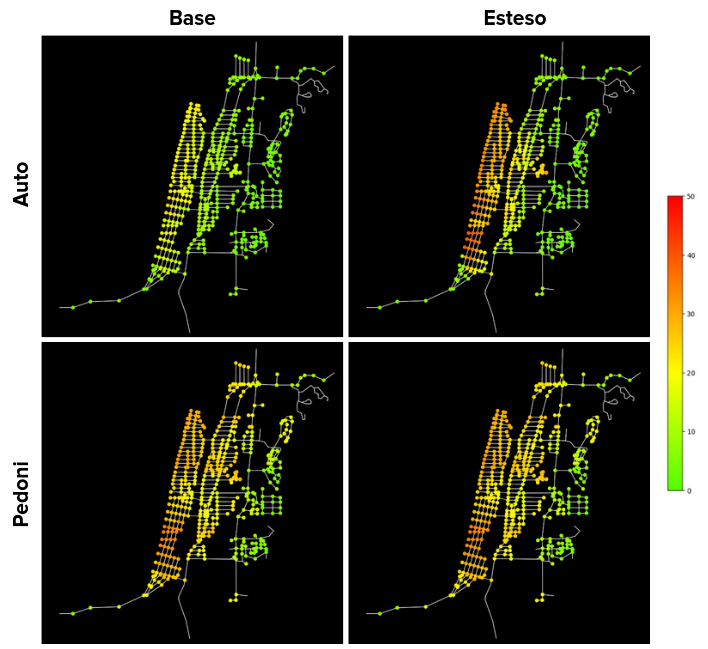
\includegraphics[width=\textwidth]{images/analisi/comparison-evtimes-map.png}
    \caption{Comparazione dei tempi di evacuazione mediati tra gli agenti che partono dallo stesso nodo della rete. }
    \label{fig:analisi-comparison-ev-times-map}
\end{figure}

\pagebreak


\subsubsection*{Flusso}
Per valutare la gestione delle intersezioni è stato considerato il flusso distinguendo tra i due tipi di intersezione.

Per ogni intersezione è stato calcolato il flusso in entrata e in uscita sommando i valori di ogni strada al variare del numero di auto e pedoni.

Come si nota nella figura \ref{fig:analisi-comparison-in-out-flow-ped},
il flusso dei pedoni non presenta particolari differenze tra modello base ed esteso, nonostante le modifiche apportate ai pedoni.

Per entrambi i modelli il flusso in entrata e in uscita in ogni intersezione è molto simile.
Inoltre all'aumentare del numero di pedoni c'è un incremento nel flusso.

%Nella maggior parte dei casi il flusso delle intersezioni TWSC risulta più basso rispetto a quelle AWSC, poichè la strada secondaria
%è bloccata finchè la principale è occupata.

\begin{figure}[ht]
    \centering
    \begin{subfigure}{\textwidth}
        \centering
        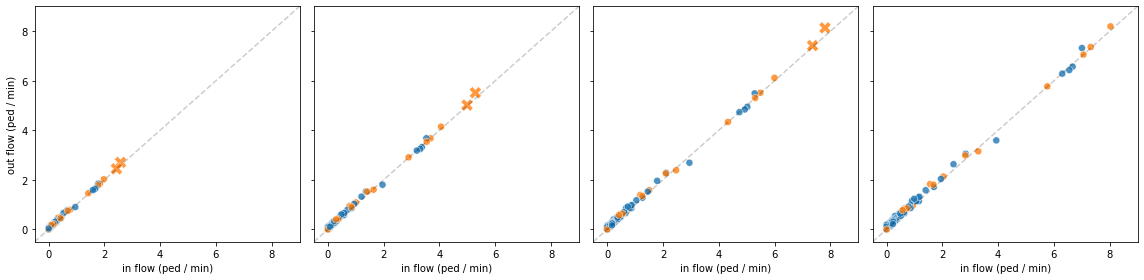
\includegraphics[width=\textwidth]{images/analisi/comparison-base-in-out-flow-ped.png}
        \caption{Modello base}
    \end{subfigure}

    \begin{subfigure}{\textwidth}
        \centering
        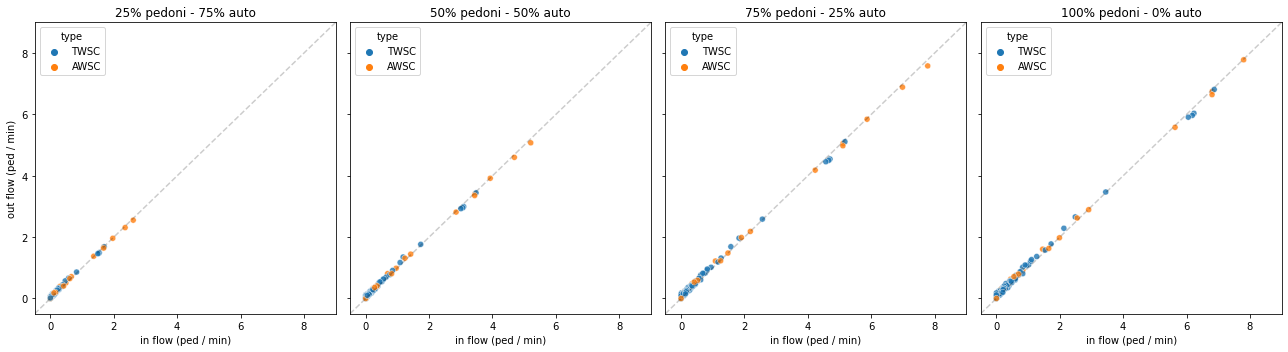
\includegraphics[width=\textwidth]{images/analisi/comparison-new-in-out-flow-ped.png}
        \caption{Modello esteso}
    \end{subfigure}
    \caption{
        Confronto tra il flusso dei pedoni in entrata e in uscita per ogni intersezione al crescere del numero di pedoni.
    }
    \label{fig:analisi-comparison-in-out-flow-ped}
\end{figure}

Osservando il flusso delle auto (Fig. \ref{fig:analisi-comparison-in-out-flow-car})
viene riscontrato un leggero incremento di flusso in entrata all'aumentare del numero di auto.
Il flusso in entrata e in uscita non sono perfettamente bilanciati e risultano più sparsi rispetto al flusso dei pedoni.
Inoltre in molte intersezioni il flusso in entrata è maggiore del flusso in uscita.

Nel modello esteso il flusso risulta più basso
probabilmente a causa della gestione delle intersezioni che genera una diminuzione del traffico in uscita che,
propagandosi in tutta la rete, abbassa il flusso in tutte le intersezioni.

\begin{figure}[ht]
    \centering
    \begin{subfigure}{\textwidth}
        \centering
        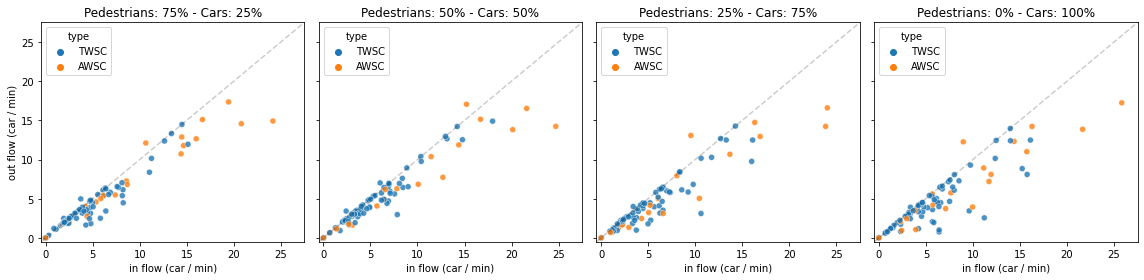
\includegraphics[width=\textwidth]{images/analisi/comparison-base-in-out-flow-car.png}
        \caption{Modello base}
    \end{subfigure}

    \begin{subfigure}{\textwidth}
        \centering
        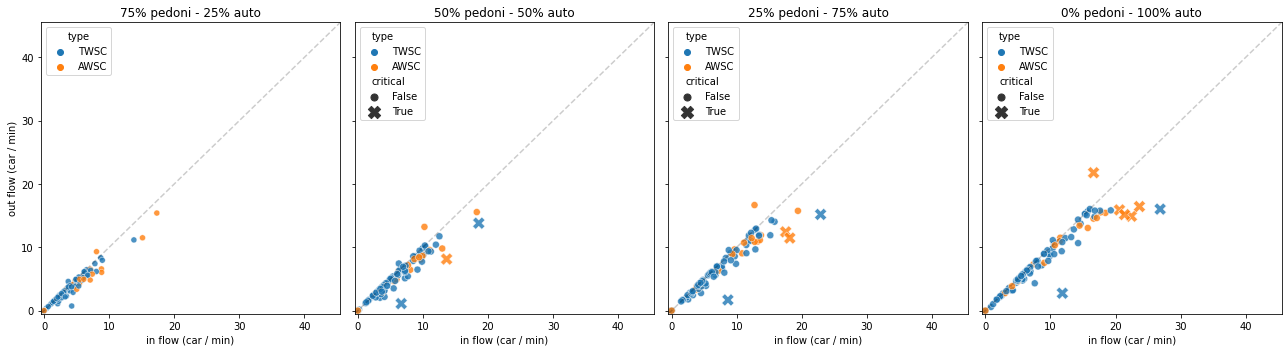
\includegraphics[width=\textwidth]{images/analisi/comparison-new-in-out-flow-car.png}
        \caption{Modello esteso}
    \end{subfigure}
    \caption{
        Confronto tra il flusso delle auto in entrata e in uscita per ogni intersezione al crescere del numero di auto.
    }
    \label{fig:analisi-comparison-in-out-flow-car}
\end{figure}

\pagebreak



\subsection{Comparazione con Z. Wang e Jia (2021)}
In questa sezione verranno comparati il modello base e il modello esteso con il modello di \textcite{wang2021novel},
il quale rappresenta un modello recente allo stato dell'arte e considera lo stesso scenario di evacuazione di questo lavoro.

\textcite{wang2021novel} hanno effettuato 4000 simulazioni con 5000 agenti e
hanno modellato l'incertezza della percentuale di auto con una variabile $p_c \sim N(\mu_c, \sigma_c)$ troncata in (0, 1),
dove $\mu_c$ segue una distribuzione uniforme in [0, 1] e $\sigma_c$ = 0.15.
Inoltre sono stati considerati diversi casi che introducono o meno diverse caratteristiche nel modello (Tab. \ref{tab:cases}).

\begin{table}[ht]
    \centering
    \begin{tabular}{|c|c|c|c|}
        \hline
        Cases & Seismic damage & Pedestrian-vehicle interaction & Speed adjustment \\ \hline
        C0    & No             & No                             & No               \\ \hline
        C1    & No             & No                             & Yes              \\ \hline
        C2    & No             & Yes                            & Yes              \\ \hline
        C3    & Yes            & No                             & Yes              \\ \hline
        C4    & Yes            & Yes                            & Yes              \\ \hline
    \end{tabular}
    \caption{Casi di simulazione del modello \textcite{wang2021novel}.}
    \label{tab:cases}
\end{table}

Per comparare con il modello di \textcite{wang2021novel} sono state mediate le prove effettuate al variare del numero
di auto e di pedoni (Fig. \ref{fig:analisi-comparison-wang2}).
Nella comparazione verranno presi in considerazione esclusivamente i casi C0, C1 e C2, ovvero quelli
che non gestiscono i danni sismici (Fig. \ref{fig:analisi-comparison-wang1}).

\begin{figure}[p]
    \centering
    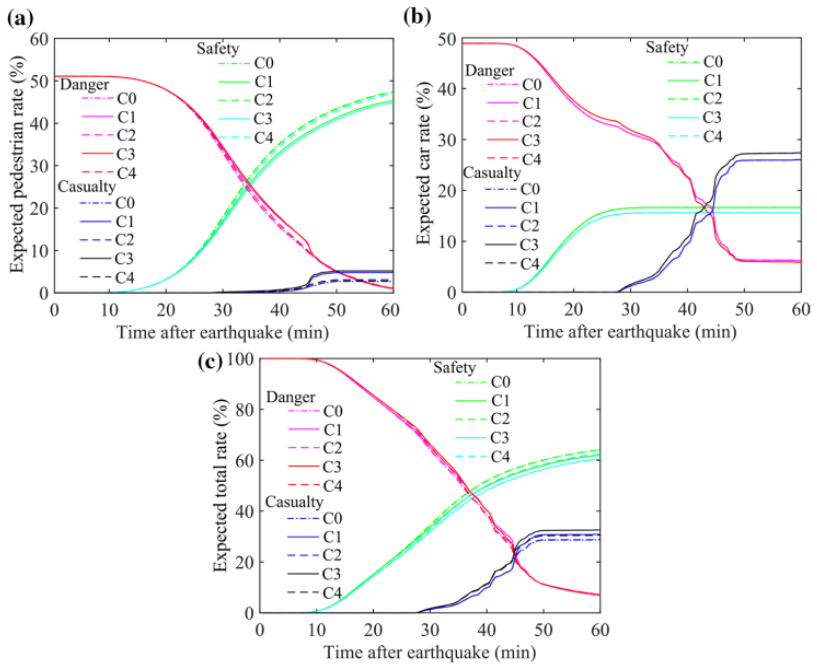
\includegraphics[width=0.8\textwidth]{images/analisi/WANG_comparison1.png}
    \caption{Confronto della percentuali di evacuati e di vittime per auto, pedoni e totale per il modello di \textcite{wang2021novel}.}
    \label{fig:analisi-comparison-wang1}
\end{figure}

\begin{figure}[p]
    \centering
    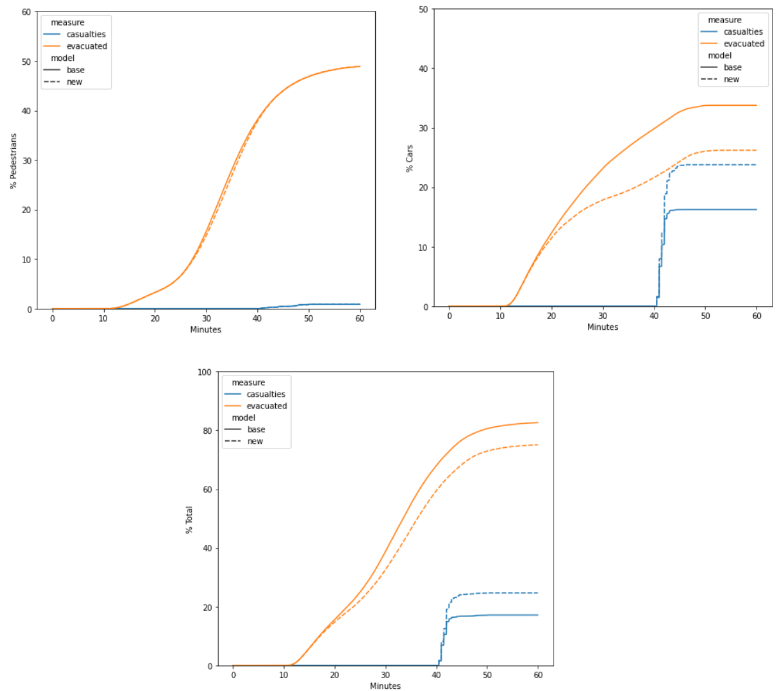
\includegraphics[width=0.8\textwidth]{images/analisi/WANG_comparison2.png}
    \caption{Confronto della percentuali di evacuati e di vittime per auto, pedoni e totale per modello base ed esteso.}
    \label{fig:analisi-comparison-wang2}
\end{figure}

Una delle prime differenze tra i due modelli riguarda il tempo di preparazione. Infatti i primi agenti nel modello di
\textcite{wang2021novel} iniziano a evacuare intorno ai 10 minuti, mentre nel modello esteso e nel modello base iniziano
dopo 1 minuto.

Nel modello di \textcite{wang2021novel} le prime vittime si verificano a circa 28 minuti ovvero quando lo tsunami inizia ad arrivare alla costa,
mentre nel modello esteso e nel modello base poco prima dei 40 minuti, ovvero quando lo tsunami ha già coperto l'area vicino alla costa.
Dopo 50 minuti lo tsunami ha raggiunto la massima distanza e infatti in tutti i modelli il numero di vittime rimane costante.

Osservando solo i pedoni si può notare come il caso C2 sia lo scenario più simile ai risultati
ottenuti dal modello base ed esteso per vittime ed evacuati, con valori leggermente inferiori di evacuati e maggiori di vittime,
nonostante varie differenze tra i due modelli.

Inoltre nel modello di \textcite{wang2021novel} si nota una differenza significativa
tra il caso con la velocità costante (C0) e il caso con velocità variabile (C1),
rispetto alla differenza tra il modello base ed esteso.

In tutti i modelli le auto presentano differenze più marcate sia per le vittime che per gli evacuati.
Nel modello di \textcite{wang2021novel} gli evacuati hanno una curva crescente fino a circa 30 minuti dopo i quali si appiattisce e raggiunge un valore di circa 17\%,
mentre nel modello base e nel modello esteso la curva continua a crescere fino intorno ai 40 minuti e raggiunge un valore di 87\% nel modello base e di 79\% nel modello esteso.

Per quanto riguarda le vittime nel modello di \textcite{wang2021novel} l'andamento cresce lentamente tra 28 e circa 50 minuti raggiungendo un valore di 26\%, mentre nel
modello base e nel modello esteso la maggior parte delle vittime è concetrata vicino a 40 minuti raggiungendo un valore di di 12\% nel modello base e di 21\% nel modello esteso.

Nel caso totale sono presenti andamenti simili a quelli già descritti nei grafici per i pedoni e per le auto, ovvero sia il modello base ed il modello esteso
prevedono un numero maggiore di evacuati e un numero minore di vittime rispetto al modello di \textcite{wang2021novel}.

Il modello esteso risulta più ottimistico per evacuati e vittime rispetto al modello di \textcite{wang2021novel} nonostante la gestione delle intersezioni
che prevede un rallentamento del traffico e più vittime rispetto al modello base.


\begin{table}[ht]
    \centering
    \begin{tabular}{|l|l|l|}
        \hline
                                                                                                                               & \textbf{Base / Esteso}          & \textbf{Wang et. al 2021} \\ \hline
        \textbf{N° agenti}                                                                                                     & 4502                            & 5000                      \\ \hline
        \textbf{Pedoni}                                                                                                        &
        \begin{tabular}[c]{@{}l@{}}$\mu_p$ = 1.22\\ $\sigma_p$ = 0.2\\ costante / variabile\end{tabular}                       &
        \begin{tabular}[c]{@{}l@{}}$\mu_p$ $\sim$U(1.4, 2)\\ $\sigma_p$ $\sim$U(0.1, 0.6)\\ variabile\end{tabular}                                                                           \\ \hline
        \textbf{Auto}                                                                                                          &
        \begin{tabular}[c]{@{}l@{}}1 auto = 1 agente\\ general-motors\\ $V_{max}$ = 55 km/h\end{tabular} &
        \begin{tabular}[c]{@{}l@{}}1 auto = 4 agenti\\ greenshields \\ $V_{max}$ = 40 km/h\end{tabular}                                                                \\ \hline
        \textbf{Casualty Model}                                                                                                & $H_c$ = 0.5 m                   & $H_c$ $\sim$U(0.5, 3) m   \\ \hline
        \textbf{\begin{tabular}[c]{@{}l@{}}Tempo di \\ preparazione\end{tabular}}                                              &
        \begin{tabular}[c]{@{}l@{}}$t_0$ = 0\\ $\tau$ = 1\\ $\sigma_t$ = 0.5\end{tabular}                                      &
        \begin{tabular}[c]{@{}l@{}}$t_0$ $\sim$U(3, 10)\\ $\tau$ $\sim$U(0, 10)\\ $\sigma_t$ $\sim$U(1, 5)\end{tabular}                                                                      \\ \hline
        \textbf{\begin{tabular}[c]{@{}l@{}}Probabilità \\ Pedoni / Auto\end{tabular}}                                          &
        \begin{tabular}[c]{@{}l@{}}100\% - 0\%, 75\% - 25\%, \\50\% - 50\%, 25\% - 75\%, \\0\% - 100\%\end{tabular}            &
        \begin{tabular}[c]{@{}l@{}}$\mu_c$ $\sim$U(0, 1)\\ $\sigma_c$ = 0.15\end{tabular}                                                                                                    \\ \hline
        \textbf{\begin{tabular}[c]{@{}l@{}}Interazioni \\ Auto-Pedoni\end{tabular}}                                            & nessuna / gestione intersezioni & tre fasi di traffico      \\ \hline
    \end{tabular}
    \caption{Differenze modelli base ed esteso con il modello \textcite{wang2021novel}.}
    \label{tab:differences}
\end{table}

In generale risultano abbastanza diversi se non per i pedoni che sono modellati in modo simile, il tutto dovuto da molti fattori (Tab. \ref{tab:differences}),
specialmente i tempi di partenza e il numero di auto considerate le quali sono molto influenti sul numero di evacuati e vittime.

\pagebreak
